% This must be in the first 5 lines to tell arXiv to use pdfLaTeX, which is strongly recommended.
\pdfoutput=1
% In particular, the hyperref package requires pdfLaTeX in order to break URLs across lines.

\documentclass[11pt]{article}

% Change "review" to "final" to generate the final (sometimes called camera-ready) version.
% Change to "preprint" to generate a non-anonymous version with page numbers.
\usepackage[final]{acl}

% Standard package includes
\usepackage{times}
\usepackage{latexsym}

% For proper rendering and hyphenation of words containing Latin characters (including in bib files)
\usepackage[T1]{fontenc}
% For Vietnamese characters
% \usepackage[T5]{fontenc}
% See https://www.latex-project.org/help/documentation/encguide.pdf for other character sets

% This assumes your files are encoded as UTF8
\usepackage[utf8]{inputenc}

% This is not strictly necessary, and may be commented out,
% but it will improve the layout of the manuscript,
% and will typically save some space.
\usepackage{microtype}

% This is also not strictly necessary, and may be commented out.
% However, it will improve the aesthetics of text in
% the typewriter font.
\usepackage{inconsolata}

%Including images in your LaTeX document requires adding
%additional package(s)
\usepackage{graphicx}
\usepackage{subcaption}

\usepackage{acronym}
\usepackage[inline]{enumitem}
\usepackage{booktabs}
\usepackage{tabularx}
% MUST BE THE LAST IMPORT
\usepackage{cleveref}

\acrodef{gnn}[GNN]{Graph Neural Network}

\newcommand{\meta}[1]{{\color{blue}#1}}

% If the title and author information does not fit in the area allocated, uncomment the following
%
%\setlength\titlebox{<dim>}
%
% and set <dim> to something 5cm or larger.

\title{Graph Neural Network Project \\
Bertinoro International Spring School (BISS) 2024}

% Author information can be set in various styles:
% For several authors from the same institution:
% \author{Martina Baiardi \and Davide Domini \and Nicolas Farabegoli \and Alessandro Petrella \and Gianni Tumedei }
%         Address line \\ ... \\ Address line}
% if the names do not fit well on one line use
%         Author 1 \\ {\bf Author 2} \\ ... \\ {\bf Author n} \\
% For authors from different institutions:
% \author{Author 1 \\ Address line \\  ... \\ Address line
%         \And  ... \And
%         Author n \\ Address line \\ ... \\ Address line}
% To start a separate ``row'' of authors use \AND, as in
% \author{Author 1 \\ Address line \\  ... \\ Address line
%         \AND
%         Author 2 \\ Address line \\ ... \\ Address line \And
%         Author 3 \\ Address line \\ ... \\ Address line}


\author{
  Martina Baiardi \\
  University of Bologna \\
  {\bf m.baiardi@unibo.it} \\ \And
  Davide Domini \\
  University of Bologna \\
  {\bf davide.domini@unibo.it} \\  \And
  Nicolas Farabegoli \\
  University of Bologna \\
  {\bf nicolas.farabegoli@unibo.it} \\  \AND
  Alessandro Petrella\\
  University of Bologna \\
  {\bf alessandro.petrella@unibo.it} \\ \And
  Gianni Tumedei \\
  University of Bologna \\
  {\bf gianni.tumedei2@unibo.it}
}

\begin{document}

\maketitle

\begin{abstract}

Online platforms for products and services - such as Spotify, Netflix, and Amazon - 
host vast product inventories and cater to millions of users. 
Therefore, it is essential to implement an optimized automated system that effectively 
recommends products aligned with users' tastes and preferences.  
%
\acp{gnn} show great promise for this purpose, and in this paper, 
we introduce a technique to develop a recommender system based on 
link prediction in heterogeneous graphs, using the MovieLens 100K dataset.
%
We provide details about the adopted architecture, the model configuration and the training
process adopted in our experiments.
%
%\meta{Briefly summarise the finding of the experiments}
Results show that our proposed model ....

\end{abstract}

\section{Task description}\label{sec:task-description}
Link prediction tasks involve predicting the existence, formation, 
or strength of a connection (or link) between two nodes in a network or graph. 
These tasks are crucial in various domains where understanding or forecasting the relationships 
between entities is important. 
In this paper we present a model based on a link prediction to implement a recommender system of movies for users.
The goal is to predict whether a user will likely enjoy a film they haven't yet seen, 
enabling the system to recommend it to them, or exclude it if it's unlikely to match their preferences.


\section{Dataset description}\label{sec:dataset-description}
The MovieLens 100k dataset is a widely-used benchmark dataset in the field of recommender systems and machine learning research. 
Released by the GroupLens Research lab, the dataset contains 100,000 ratings from 943 users on 1,682 movies, 
captured between September 19, 1997, and April 22, 1998. 
Each user in the dataset has rated at least 20 movies, with ratings ranging from 1 to 5, where 1 indicates the lowest rating and 5 the highest.
In addition to the ratings, the dataset includes demographic information for each user, 
such as age, gender, occupation, and zip code, as well as basic metadata for each movie, including title, release year, and genre. 
The dataset is structured into several files, with the primary ones being u.data (which contains the actual ratings), 
u.user (which contains user information), and u.item (which contains movie information).
The MovieLens 100k dataset is particularly valuable for researchers because of its size and the inclusion of both user and item metadata, 
enabling the exploration of various collaborative filtering techniques, 
demographic-based recommendations, and hybrid recommendation strategies. 
Its moderate size allows for quick experimentation while still providing enough data to test complex algorithms, 
making it a standard reference in the field.

\section{Architecture overview}\label{sec:architecture-overview}
In this section is described at high level, the architecture shown in \ref{fig:architecture} used to adress 
the link prediction task. 
For this purpose, is utilized \acp{gnn} with heterogeneous graphs 
as input. \Cref{fig:architecture} Shows the main architecture of the \acp{gnn}. 
A heterogeneous graph consists of nodes and edges of different types, 
each with distinct properties, unlike homogeneous graphs where all nodes and edges are 
uniform. In our case, the heterogeneous graph is composed of two types of nodes: 
users and movies, connected by a single type of edge that represents the relationship "user-rates-movie."

Before feeding the graph into the \acp{gnn}, pre-processing is performed to 
generate node embeddings. These embeddings create real-valued vectors for each node, 
capturing both the structural and semantic features of the graph.

The \acp{gnn} architecture consists of two layers, each followed by a ReLU activation 
function to introduce non-linearity. The third and final layer is a binary classifier 
designed to predict the presence or absence of edges, enabling link prediction within the 
graph.



\begin{figure*}
  \centering
  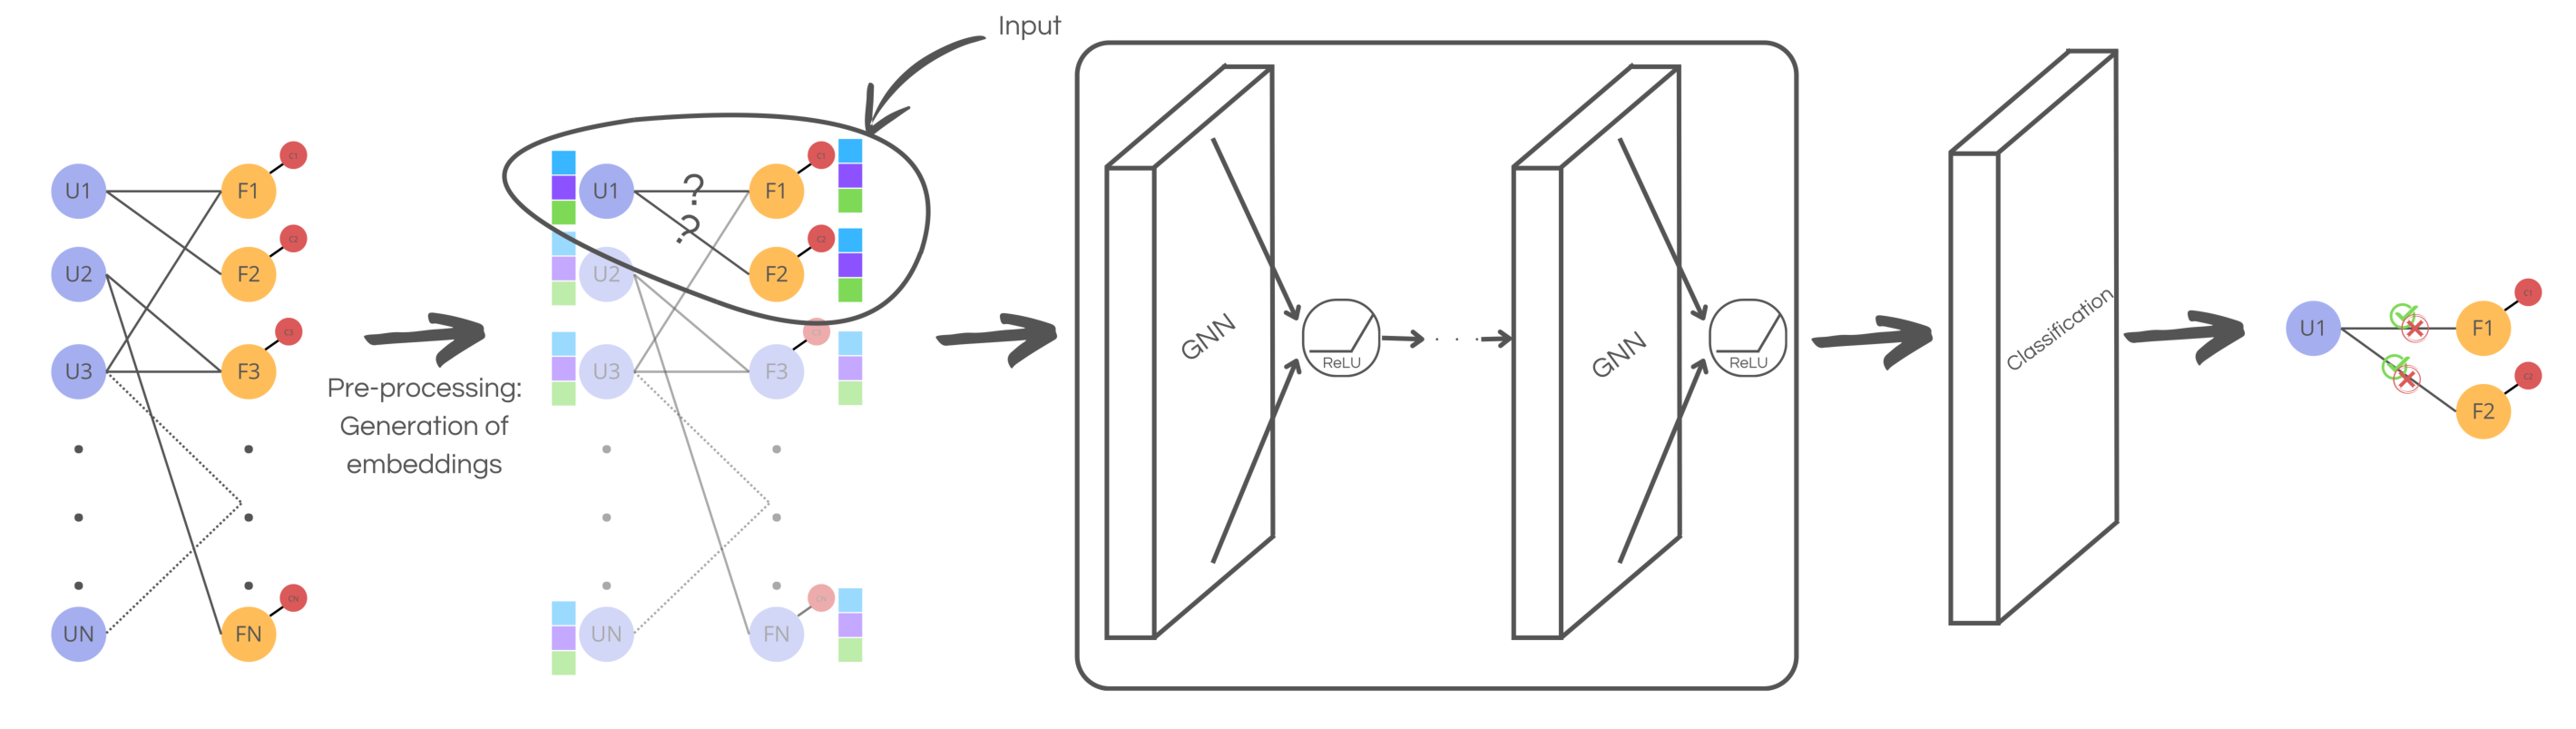
\includegraphics[width=1\linewidth]{figures/architecture.pdf}

  \caption{
    Architecture
  }
  \label{fig:architecture}
\end{figure*}

\section{Experimental setup}\label{sec:experimental-setup}

\subsection{Preprocessing}\label{sec:preprocessing}
The preprocessing stage is a fundamental part in preparing the dataset for fine-tuning a \ac{llm}.
%
This process ensures that the data is clean, consistent, and in a format suitable for the next stages.
%
The same preprocessing procedure has been applied for both the models taken into account in \Cref{sec:model-config}.
%
In the following,
we report the steps we adopted for the preprocessing stage.

\paragraph{Dataset exploration}
We used Pandas~\cite{reback2020pandas} to build a DataFrame from the CSV dataset files,
for extracting information and data manipulation.

Preliminary,
a dataset exploration is performed to understand the categorical labels' distribution,
and the posts' length provided in the dataset.
%
\Cref{fig:class-frequency} depicts the class distribution for the \emph{training set} (left chart),
and the \emph{test set} (right chart).
%
Notably,
both the classes for the training and test set are well-balanced,
requiring no rebalancing countermeasure.

Another aspect we are interested in is the post length distribution,
since we are limited in the number of token each model can accept.
%
\Cref{fig:words-distribution} shows the distribution of the posts' length divided by training and test set.
%
The two upper charts provide the distribution on the raw post of both the dataset,
while the two lower charts describe the distribution after the cleanup step (that we will discuss in the next paragraph).
%
As can be observed,
the majority of the posts are concentrated in the range $0-500$ words,
meaning that the most of the dataset will not be truncated when input to the model.
%
The posts' cleanup process do not significantly impact the length distribution of the posts in the datasets.

\paragraph{Text cleaning}
To remove noise from the input data,
we processed the raw posts to remove any irrelevant content for the model's fine-tuning.
%
In particular,
we conducted the following operations:
\begin{enumerate*}[label=(\roman{*})]
  \item remove all the extra space;
  \item remove HTML tags and special characters like \texttt{@};
  \item remove all the http links; and
  \item remove all the \texttt{\#} but preserving the text associated to the hashtag.
\end{enumerate*}
Then,
the dataset is updated with the cleaned version of the posts,
preserving the same file structure.


\begin{figure*}
  \centering
  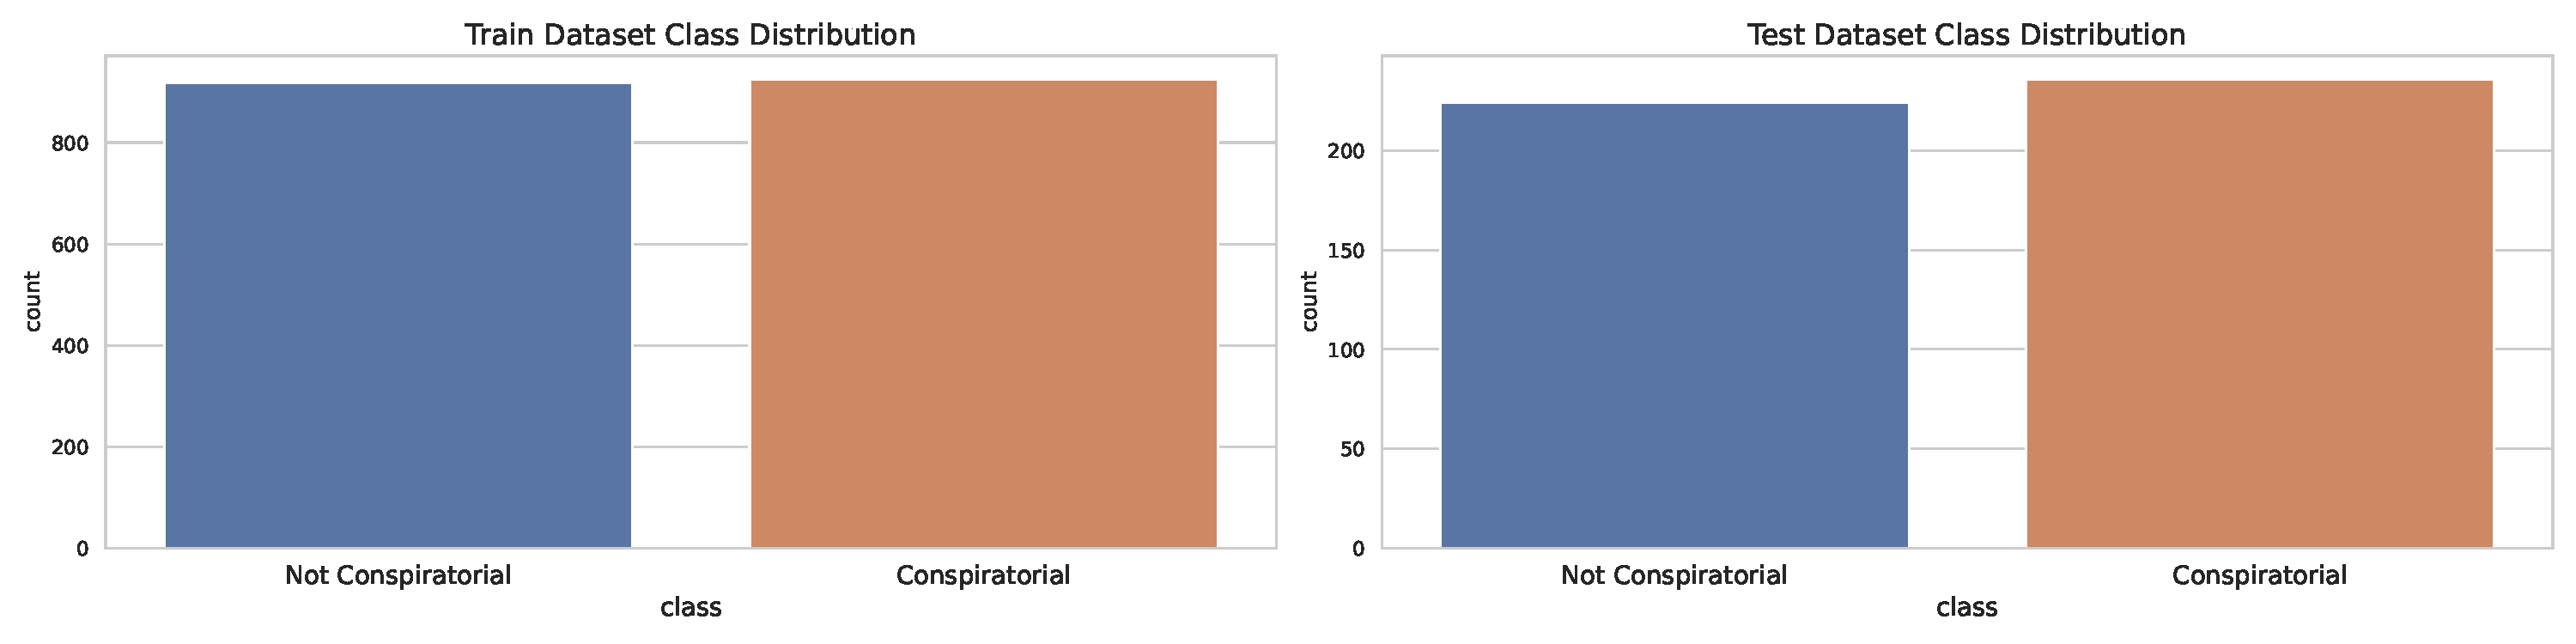
\includegraphics[width=\textwidth]{figures/class_distribution.pdf}
  \caption{
    Class distribution between the \emph{training set} and the \emph{test set}.
  }
  \label{fig:class-frequency}
\end{figure*}

\begin{figure*}
  \centering
  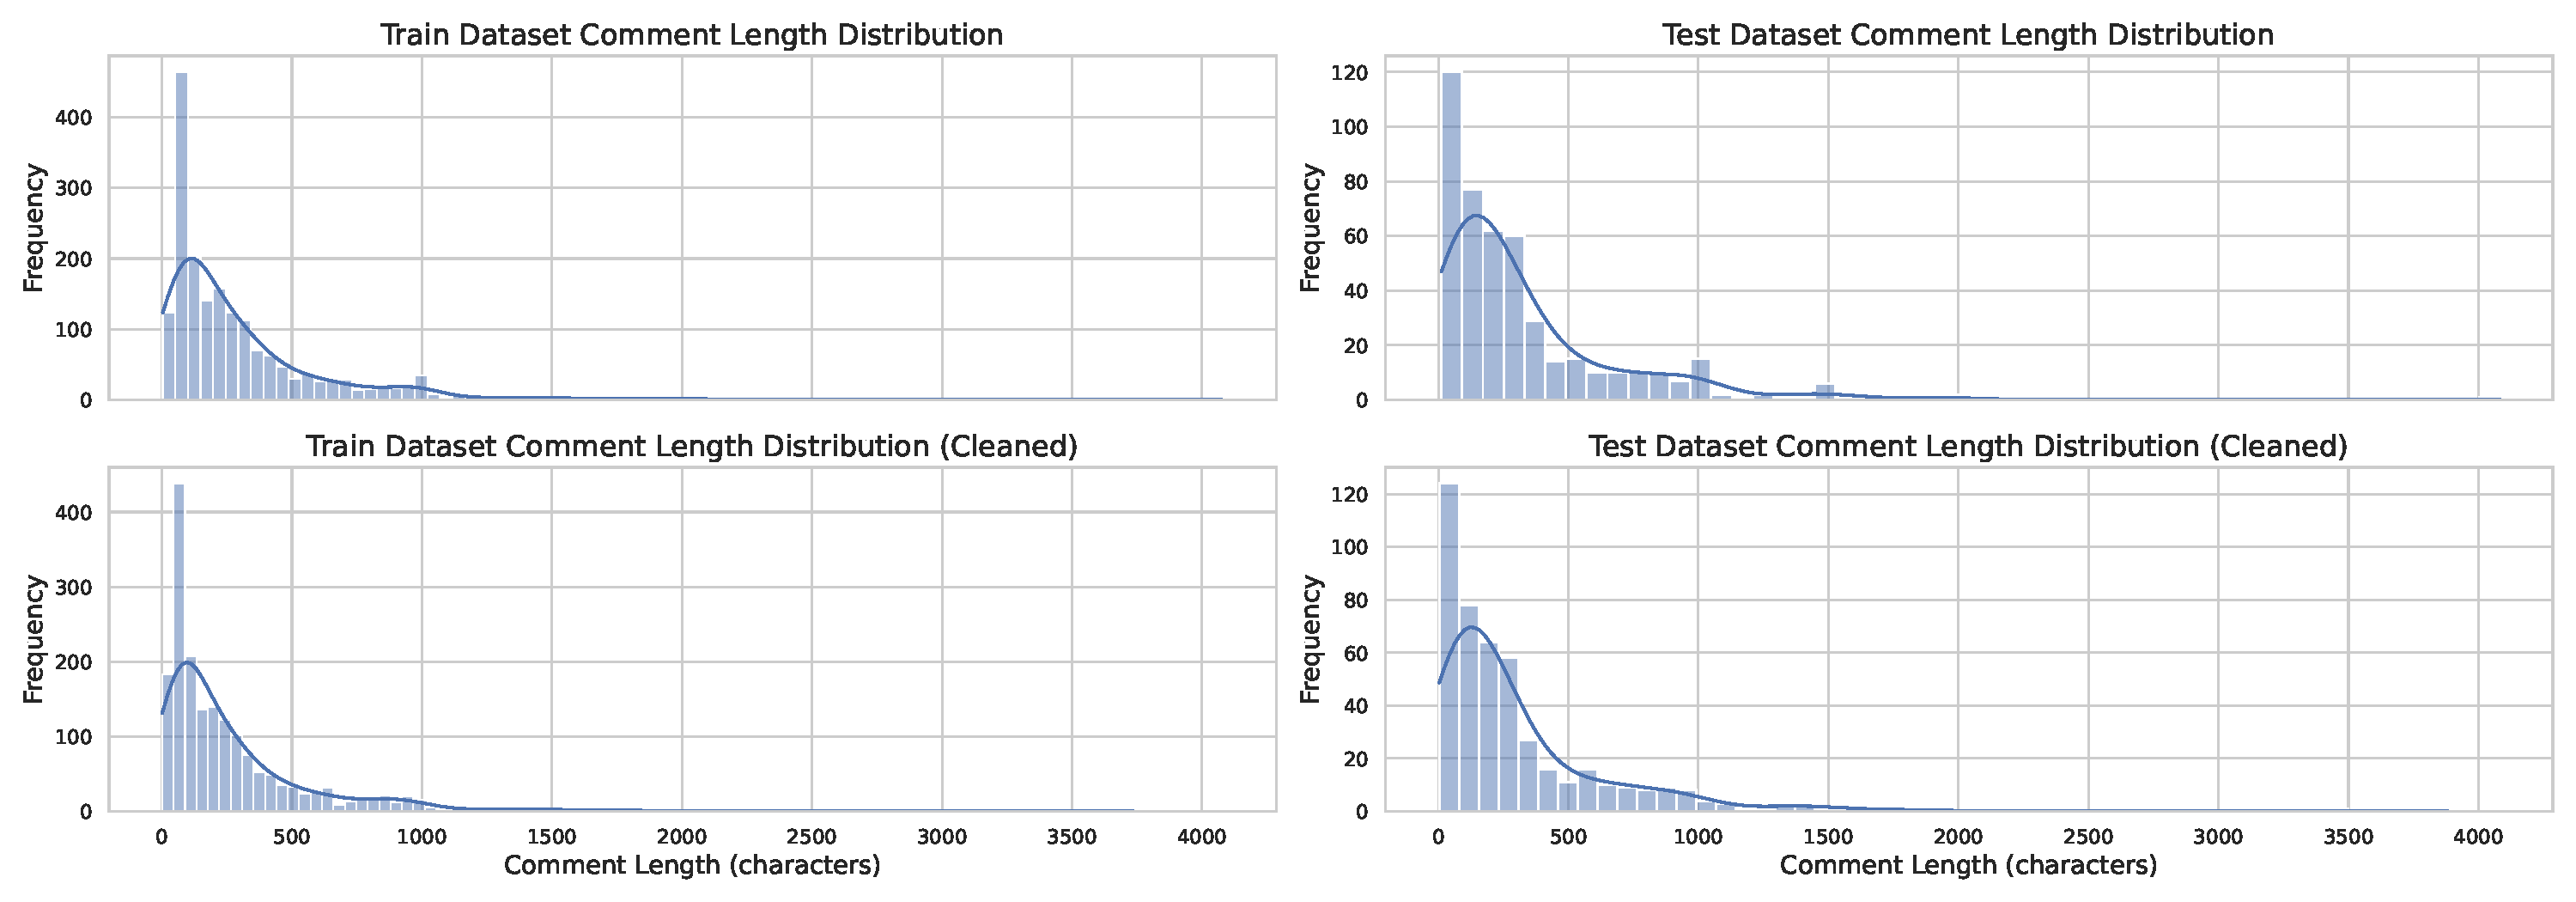
\includegraphics[width=\textwidth]{figures/comment_length_distribution.pdf}
  \caption{
    Comment length distribution for both the training dataset (on the left) and test dataset
    (on the right).
    %
    The upper charts refer to the raw content of posts, coming from the original dataset;
    in the lower charts, our cleanup preprocessing has been applied to the content.
  }
  \label{fig:words-distribution}
\end{figure*}

\subsection{Model configuration}\label{sec:model-config}
While solving ACTI-A subtask, we also compared performances of two different Transformer-based architectures,
the first one based on an \emph{Encoder} neural network, and the second one on a \emph{Decoder} neural network.

\paragraph{Encoder}

We adopted a RoBERTa-based Language Model named \texttt{UmBERTo Commoncrawl Cased},
which is trained on the large italian subcorpus of \texttt{OSCAR project} ~\footnote{\url{https://oscar-project.org/}}.
%
To address the chosen challenge, we added to this model a final layer for classification,
which returns a value for each class specified,
in our case two classes, for identifying if a text is conspiratorial or not.

Before training the model on our task we performed preprocessing, as described in \Cref{sec:preprocessing},
and then tokenization (\Cref{fig:preprocessing-and-tokenization-encoder}).
%
Concerning tokenization, \texttt{CamembertTokenizerFast} is adopted,
it normalizes strings input both regarding delimeters of the text,
but also adds a left-side padding where the input is smaller than the maximum sequence length,
that we fixed at $ 256 $ characters.
%
\begin{figure}
  \centering
  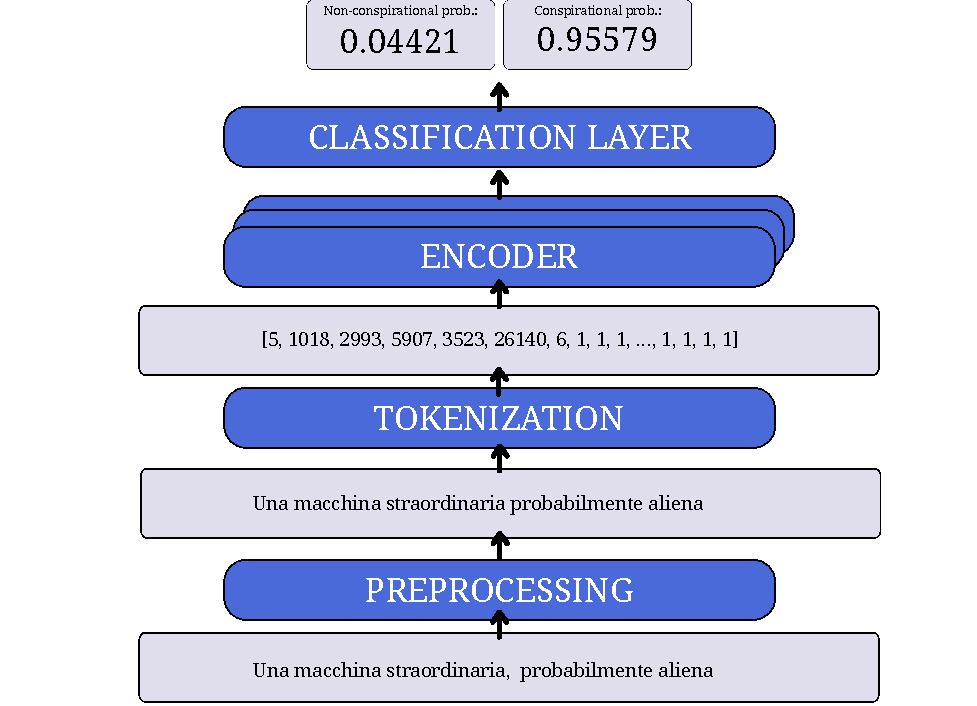
\includegraphics[width=\linewidth]{figures/encoder.pdf}
  \caption{
    Input manipulation before passing it to the encoder LLM model.
    The image exemplifies the manipulation output obtained after the cleanup process and the application of the tokenization function.
  }
  \label{fig:preprocessing-and-tokenization-encoder}
\end{figure}

\paragraph{Decoder}

The decoder model adopted to be fine-tuned is a small \texttt{OpenAI GPT2} model adapted to italian language~\cite{de-vries-nissim-2021-good}.
%
Similarly to the encoder configuration,
text is preprocessed and then tokenized before being served to the model.
%
Oppositely from the encoder,
text tokenization is performed using \texttt{GPT2Tokenizer}
and configured to add the padding on the right side of the text input (\Cref{fig:preprocessing-and-tokenization-decoder}).
%
This is made because, given the architecture of a decoder model,
the last token of the input sequence is used to make predictions about the next token that should follow the input,
this means that the last token of the input sequence contains all the information needed in the prediction.
%
\begin{figure}
  \centering
  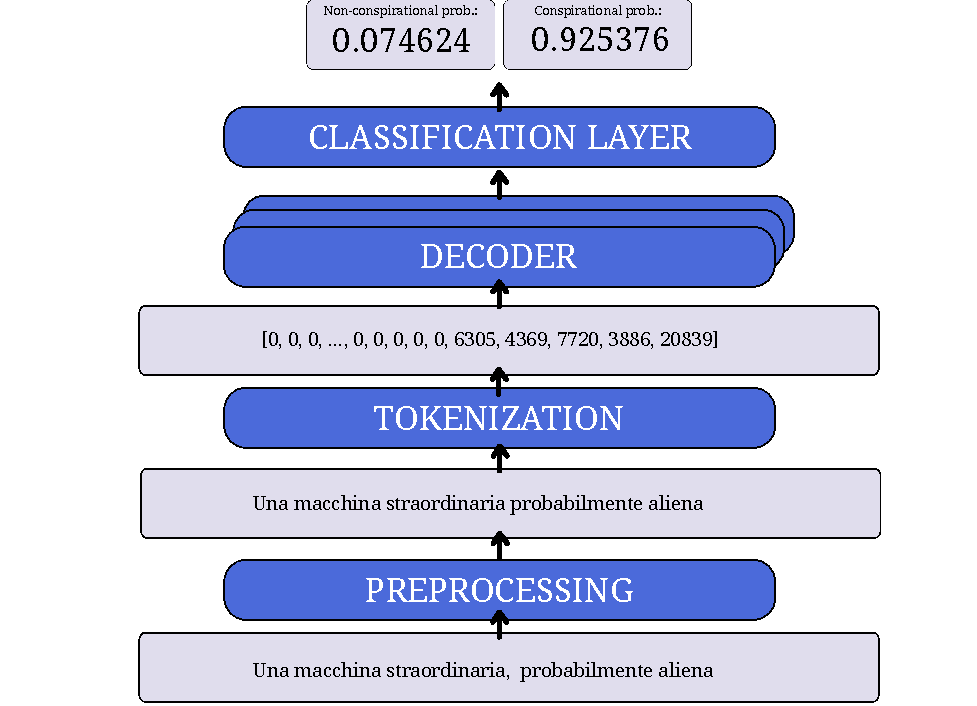
\includegraphics[width=\linewidth]{figures/decoder.pdf}
  \caption{
    Input manipulation before passing it to the decoder LLM model.
    The image exemplifies the manipulation output obtained after the cleanup process and the application of the tokenization function.
  }
  \label{fig:preprocessing-and-tokenization-decoder}
\end{figure}

\subsection{Training process}\label{sec:training-process}
During the training phase, we focused on fine-tuning two distinct models: one was encoder-only and the
  other was decoder-only (as described in~\Cref{sec:model-config}).
  We leveraged the libraries PyTorch~\cite{NEURIPS2019_9015} and HuggingFace for this process.
  To maintain consistency, we applied the same hyperparameters to both models, which included:
  \begin{enumerate*}[label=(\roman{*})]
    \item $4$ epochs of fine-tuning;
    \item a maximum sequence length of $256$; and
    \item a batch size of $16$.
  \end{enumerate*}
  \meta{TODO: Discutere delle scelte forzate dal fatto che la memoria ci ha limitato nel sequebnce length e, conseguentemente, il batch size e' stato adattato.}
  The only variation was in the learning rate, where we used $2 \cdot 10^{-5}$ for the encoder and $5 \cdot 10^{-5}$ for the decoder.
  Finally, we used the cross-entropy loss.


\section{Result and analysis}\label{sec:results-analysis}

\def\arraystretch{1.2}%
\begin{table}
  \centering
  \begin{tabularx}{\columnwidth}{X r}

    \toprule
    \textit{Model} & $F_1 score$ \\
    \midrule\midrule

    \multicolumn{2}{c}{\textbf{Baseline}} \\
    \midrule
    Kaggle Baseline & $0.5107$    \\
    EVALITA Winner &   $0.8572$  \\
    
    \midrule
    \multicolumn{2}{c}{\textbf{Proposed model with no fine-tuning}} \\
    \midrule
    
    Encoder-Only &  $0.4538$    \\
    Decoder-Only &   $0.3189$  \\
    
    \midrule
    \multicolumn{2}{c}{\textbf{Proposed model after fine-tuning}}\\
    \midrule
    
    Encoder-Only &  $0.8211$    \\
    Decoder-Only &   $0.7464$  \\
    \bottomrule
  \end{tabularx}

  \caption{\label{table:results}
    Results obtained from the models proposed, with and without fine-tuning, 
    on ACTI-A subtask. Baseline were provided by the ACTI task organizers via Kaggle.
  }
\end{table}

We evaluated the performance of our classification models using the $F_1 score$. 
Table \ref{table:results} displays the performance of our proposed model, 
along with additional scores for comparison to provide further insights into the results. 
The $F_1 scores$ were computed on the labeled test set provided by the organizers of the ACTI task.
The Kaggle baseline $F_1 scores$ is 0.5107, while the EVALITA winners achieved 0.8572. 
Our initial models, without any tuning, achieved $F_1 scores$ of 0.4538 and 0.3189 for the encoder-only 
and decoder-only configurations, respectively. After fine-tuning, the $F_1 scores$ improved to 0.8211 and 0.7464.
Comparing the results, we observe that our proposed models significantly 
outperform the baseline ($ +0.3104 $ and $+0.2357$) but do not reach the performance level of the EVALITA winners.
Figure \ref{fig:confusion-matrix} shows the confusion matrices resulting from 
the test set classifications for both proposed models. 
Encoder-only matrix indicates that this model has a good 
performance in identifying "Conspiratorial" instances but has some difficulties in 
correctly identifying "Non-Conspiratorial" instances, as evidenced by the number of false positives. 
Instead, examining the decoder-only matrix, we observe that the number of false positives 
remains similar to the encoder-only model. However, the number of false negatives increases 
significantly, surpassing the number of false positives. 
This increased difficulty in correctly identifying positive instances 
results in a lower $F_1 score$ for the decoder-only model.


% \begin{figure}
%   \centering
%   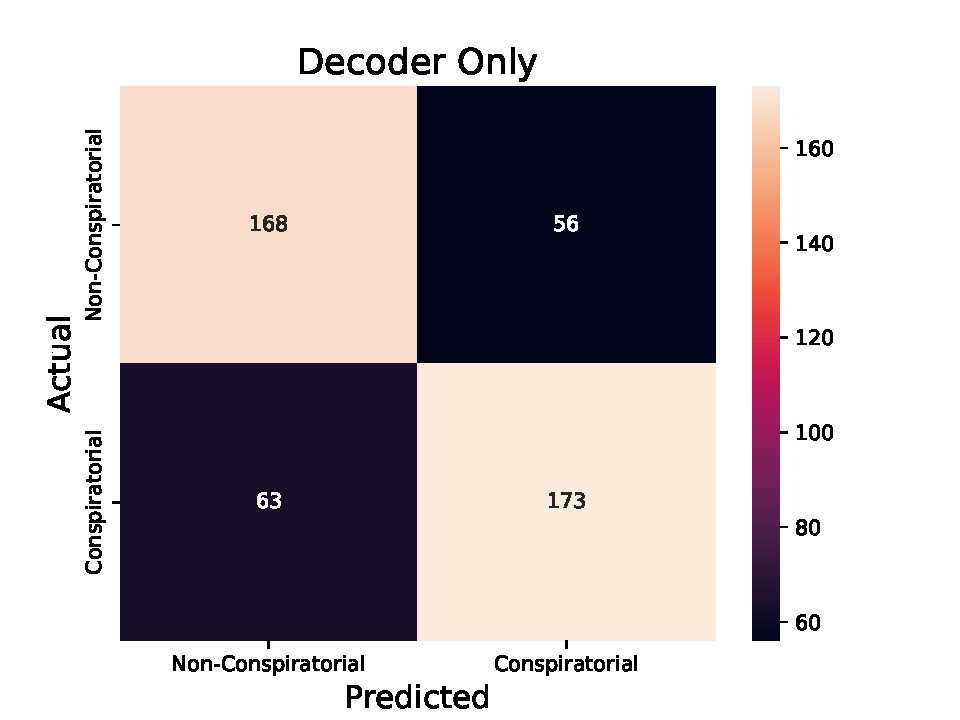
\includegraphics[width=\columnwidth]{figures/decoder-only-confusion-matrix.pdf}
%   \caption{
%    TBA}
%   \label{fig:decoder-only-cm}
% \end{figure}

% \begin{figure}
%   \centering
%   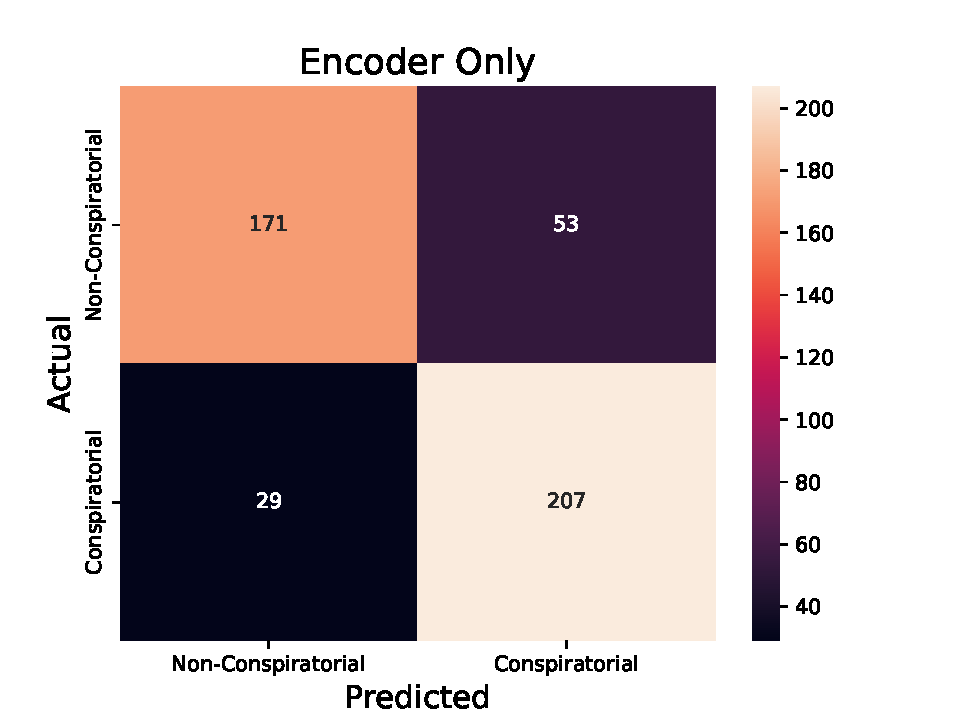
\includegraphics[width=\columnwidth]{figures/encoder-only-confusion-matrix.pdf}
%   \caption{
%    TBA}
%   \label{fig:encoder-only-cm}
% \end{figure}


\begin{figure}
    \centering
    \begin{subfigure}{\columnwidth}
        \centering
        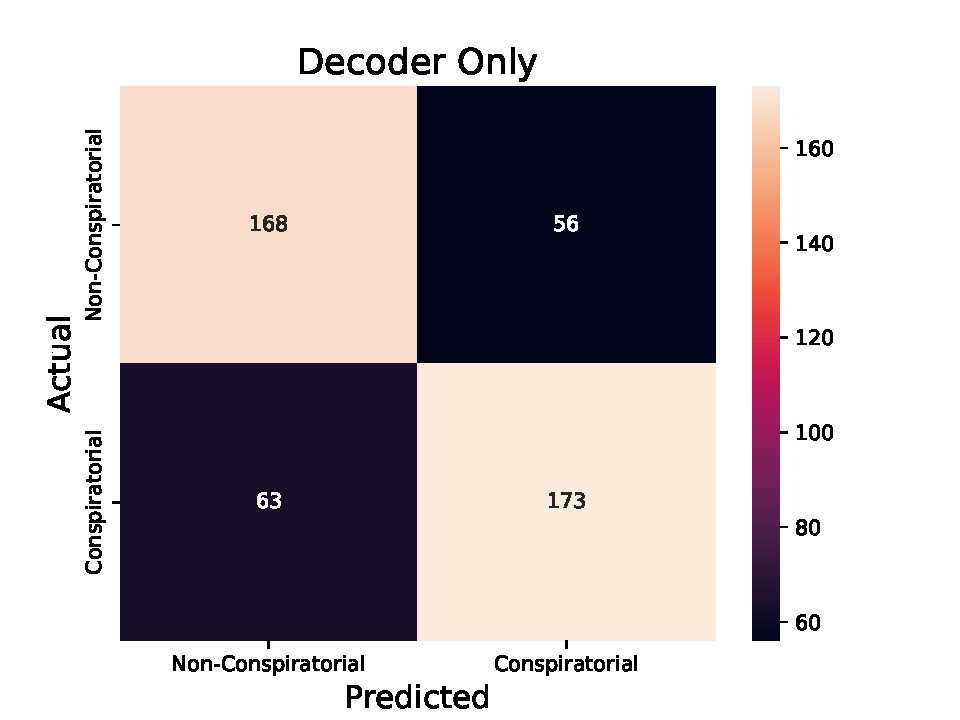
\includegraphics[width=\textwidth]{figures/decoder-only-confusion-matrix.pdf}
    \end{subfigure}
    \begin{subfigure}{\columnwidth}
        \centering
        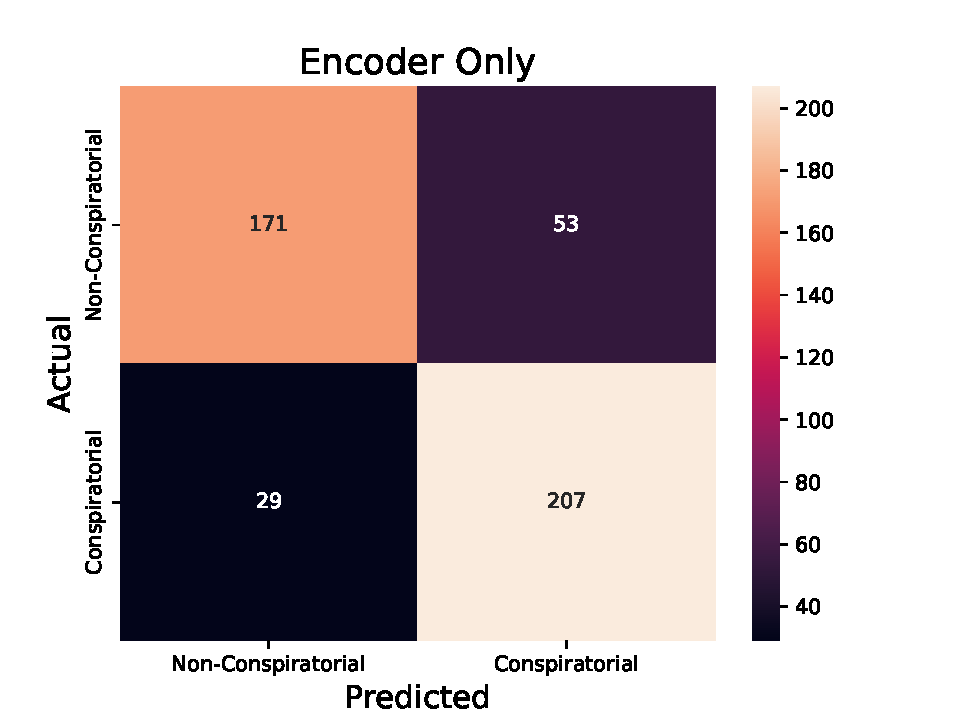
\includegraphics[width=\textwidth]{figures/encoder-only-confusion-matrix.pdf}
    \end{subfigure}
    \caption{Classification results on the test set for both encoder-only and decoder-only models.}
    \label{fig:confusion-matrix}
\end{figure}


\bibliography{bibliography}

% \appendix

% \section{Example Appendix}
% \label{sec:appendix}

% This is an appendix.

\end{document}
